
\chapter{GCSE Revision - Number Questions}
Standard Form, Bounds, Percentages, Direct/Indirect Proportion, Fractions, Line Graphs, LCM.

\begin{enumerate}
  \item %
  \begin{enumerate}
    \item Write $7.8 \time 10^{-4}$ as an ordinary number.\mrk{1}\\[2cm]\vspace*{0pt}\hfill\dline
    \item Write $95 600 000$ as a number in standard form.\mrk{1}\\[2cm]\vspace*{0pt}\hfill\dline
  \end{enumerate}
  \lmrk{1}{2}
  \item In a sale normal prices are reduced by $20\%$. A washing machine has a sale price of $\pounds 464$. By how much money is the normal price of the washing machine reduced?\mrk{3}\\[4cm]\vspace*{0pt}\hfill\pounds\dline
  \item $y$ is directly proportional to the square of $x$. When $x = 3,\ y = 36$. Find the value of $y$ when $x = 5$.\mrk{4}\\[2cm]\vspace*{0pt}\hfill\dline
  \item %
  $$
  m = \frac{\sqrt{s}}{t}
  $$
  $s = 3.47$ correct to $2$ decimal places.\\
  $t = 8.132$ correct to $3$ decimal places.\par 
  By considering bounds, work out the value of $m$ to a suitable degree of accuracy. You must show all your working and give a reason for your final answer.\\[3cm]\vspace*{0pt}
  \item %
  \begin{enumerate}
    \item Write $8.2 \times 10^5$ as an ordinary number.\mrk{1}\\[1.5cm]\vspace*{0pt}\hfill\dline
    \item Write $0.000376$ in standard form.\mrk{1}\\[1.5cm]\vspace*{0pt}\hfill\dline
    \item Work out the value of $(2.3 \times 10^{12}) \divisionsymbol (4.6 \times 10^3)$. Give your answer in standard form.\mrk{2}\\[2cm]\vspace*{0pt}\hfill\dline
  \end{enumerate}
  \lmrk{5}{4}
  \item $h$ is inversely proportional to the square of $r$. When $r = 5,\ h = 3.4$. Find the value of $h$ when $r = 8$.\mrk{3}\\[2.5cm]\vspace*{0pt}\hfill$h=$\dline
  \item Dan does an experiment to find the value of $\pi$. He measures the circumference and the diameter of a circle. He measures the circumference, $C$, as $170$ mm to the nearest millimetre. He measures the diameter, $d$, as $54$ mm to the nearest millimetre.\par 
  Dan uses $\pi = \dfrac{C}{d}$ to find the value of $\pi$. Calculate the upper bound and the lower bound for Dan's value of $\pi$.\mrk{4}\\[3cm]
  \vspace*{0pt}\hfill upper bound = \dline\\
  \vspace*{0pt}\hfill lower bound = \dline
  \item Viv wants to invest $\pounds 2000$ for $2$ years in the same bank.\\[0.5cm]
  \fbox{\parbox[c]{0.4\textwidth}{\centering
		\textbf{The International Bank}\\[0.5cm]
    Compound Interest\\[0.5cm]
    $4\%$ for the first year\\
    $1\%$ for each extra year}}\hfill
    \fbox{\parbox[c]{0.4\textwidth}{\centering
		\textbf{The Friendly Bank}\\[0.5cm]
    Compound Interest\\[0.5cm]
    $5\%$ for the first year\\
    $0.5\%$ for each extra year}}\\[0.5cm]
    At the end of 2 years, Viv wants to have as much money as possible. Which bank should she invest her $\pounds 2000$ in?\mrk{4}
    \newpage
    \item One sheet of paper is $9 \times 10^{-3}$ cm thick. Mark wants to put 500 sheets of paper into the paper tray of his printer. The paper tray is $4$ cm deep.\par 
    Is the paper tray deep enough for 500 sheets of paper? You must explain your answer.\mrk{3}\\[2cm]\vspace*{0pt}
    \item The normal price of a television is reduced by $30\%$ in a sale. The sale price of the television is $\pounds 350$ Work out the normal price of the television.\mrk{3}\\[2cm]\vspace*{0pt}\hfill$\pounds$ \dline
    \item Write the following numbers in order of size. Start with the smallest number.\mrk{2}
    $$
    0.038 \times 10^2 \qquad 3800 \times 10^{-4} \qquad 380 \qquad 0.38 \times 10^{-1}
    $$\\[2cm]\vspace*{0pt}
    \item Talil is going to make some concrete mix. He needs to mix cement, sand and gravel in the ratio $1 : 3 : 5$ by weight.\par
    Talil wants to make 180 kg of concrete mix. Talil has\par 
    \hspace*{1cm} 15 kg of cement\\
    \hspace*{1cm} 85 kg of sand\\
    \hspace*{1cm} 100 kg of gravel\par
    Does Talil have enough cement, sand and gravel to make the concrete mix?\mrk{4}
    \newpage
    \item Work out an estimate for $\dfrac{31\times 9.87}{0.509}$.\mrk{3}\\[2cm]\vspace*{0pt}
    \item The average fuel consumption ($c$) of a car, in kilometres per litre, is given by the formula
    $$
    c = \frac{d}{f}
    $$
    where $d$ is the distance travelled, in kilometres, and $f$ is the fuel used, in litres.\par 
    d = 163 correct to 3 significant figures.\\
    f = 45.3 correct to 3 significant figures.\par 
    By considering bounds, work out the value of $c$ to a suitable degree of accuracy. You must show all of your working and give a reason for your final answer.\mrk{5}\\[3cm]\vspace*{0pt}\hfill$c=$ \dline
    \item %
    \begin{enumerate}
      \item Write $6.43 \times 10^5$ as an ordinary number.\mrk{1}\\[1cm]\vspace*{0pt}\hfill\dline
      \item Work out the value of $2 \times 10^7 \times 8 \times 10^{-12}$ Give your answer in standard form.\mrk{2}\\[2cm]\vspace*{0pt}\hfill\dline
    \end{enumerate}
    \item %
    $$
    p^2 = \frac{x-y}{xy}
    $$
    $x = 8.5 \times 10^9$\\
    $y = 4 \times 10^8$\par 
    Find the value of $p$. Give your answer in standard form correct to 2 significant figures.\mrk{3}\\[3cm]\vspace*{0pt}\hfill\dline
    \item Liam invests $\pounds 6200$ for $3$ years in a savings account. He gets $2.5\%$ per annum compound interest.\par
    How much money will Liam have in his savings account at the end of $3$ years?\mrk{3}\\[3cm]\vspace*{0pt}\hfill$\pounds$\dline
    \item Express the recurring decimal $0.2\dot{8}\dot{1}$ as a fraction in its simplest form.\mrk{3}\\[2cm]\vspace*{0pt}\hfill\dline
    \item %
    \begin{enumerate}
      \item Write down the value of $10^0$.\mrk{1}\\\vspace*{0pt}\hfill\dline
      \item Write $6.7 \times 10^{-5}$ as an ordinary number.\mrk{1}\\\vspace*{0pt}\hfill\dline
      \item Work out the value of $(3 \times 10^7) \times (9 \times 10^6)$. Give your answer in standard form.\mrk{2}\\[2cm]\vspace*{0pt}\hfill\dline
    \end{enumerate}
    \lmrk{19}{4}
    \item %
    \begin{enumerate}
      \item Work out the value of $(6 \times 108) \times (4 \times 10^7)$. Give your answer in standard form.\mrk{2}\\[1.5cm]\vspace*{0pt}\hfill\dline
      \item Work out the value of $(6 \times 10^8) + (4 \times 10^7)$. Give your answer in standard form.\mrk{2}\\[1.5cm]\vspace*{0pt}\hfill\dline            
    \end{enumerate}
    \newpage
    \item Use your calculator to work out
    $$
    \sqrt{\frac{921 - 170\tan \ang{65}}{0.012 + 0.034}}
    $$
    \begin{enumerate}
      \item Write down all the figures on your calculator display. You must write your answer as a decimal.\mrk{2}\\[1.5cm]\vspace*{0pt}\hfill\dline    
    \end{enumerate}
    \item %
    \begin{enumerate}
      \item Write $82 500 000$ in standard form.\mrk{1}\\[1.5cm]\vspace*{0pt}\hfill\dline
      \item Work out $(5.2 \times 10^{-7}) \times (2.8 \times 10^{-9})$. Give your answer in standard form.\mrk{2}\\[1.5cm]\vspace*{0pt}\hfill\dline    
    \end{enumerate}
    \item $P$ is inversely proportional to $V$. When $V = 8,\ P = 5$
    \begin{enumerate}
      \item Find a formula for $P$ in terms of $V$.\mrk{3}\\[2cm]\vspace*{0pt}\hfill\dline
      \item Calculate the value of $P$ when $V = 2$.\mrk{1}\\[2cm]\vspace*{0pt}\hfill\dline
    \end{enumerate}
    \item Work out $1.83 \times 47$.
    \newpage
    \item You can use this conversion graph to change between pounds (\pounds) and dollars (\$).
    \begin{figure}[H]
      \centering
      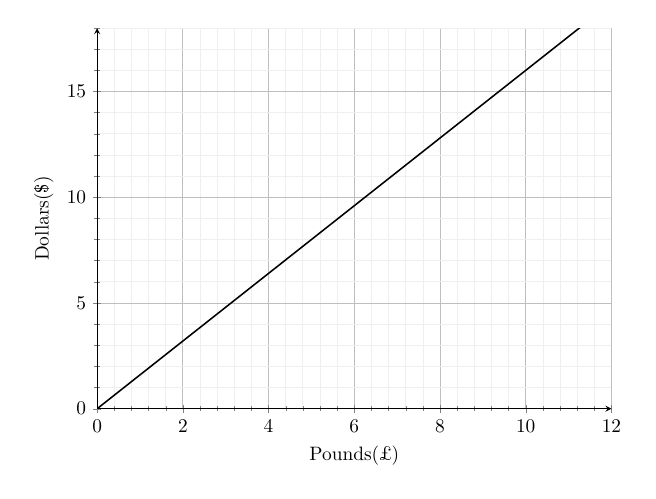
\begin{tikzpicture}[scale=0.7]
        \begin{axis}[
            xmin = 0, xmax = 12,
            ymin = 0, ymax = 18,
            grid = both,
            minor tick num = 4,
            major grid style = {lightgray},
            minor grid style = {lightgray!25},
            axis lines = left,
            width = 0.9\textwidth,
            height = 0.7\textwidth,
            xlabel = {Pounds(\pounds)},
            ylabel = {Dollars(\$)},
          ]
          % Plot a function
          \addplot[
            domain = 0:12,
            samples = 200,
            smooth,
            thick,
          ] {8/5*x};
          \end{axis}
        \end{tikzpicture}
      \end{figure}
      \begin{enumerate}
        \item Use the conversion graph to change $\pounds 5$ to dollars.\mrk{1}\\[1cm]\vspace*{0pt}\hfill\$\dline\\
        Ella has \$200 and \pounds 800. Her hotel bill is \$600. Ella pays the bill with the \$200 and some of the pounds
        \item Use the conversion graph to work out how many pounds she has left.\mrk{4}\\[1cm]\vspace*{0pt}\hfill\pounds\dline
      \end{enumerate}
      \lmrk{25}{4}
      \item Trams leave Piccadilly\par
      \hspace*{2cm} to Eccles every 9 minutes \hspace*{2cm} to Didsbury every 12 minutes\par
      A tram to Eccles and a tram to Didsbury both leave Piccadilly at 9 a.m. At what time will a tram to Eccles  and a tram to Didsbury next leave Piccadilly at the same time?\mrk{3}\\[2cm]\vspace*{0pt}\hfill\dline
      \item Given that	$1793 \times 185 = 331 705$. Write down the value of
      \begin{enumerate}
        \item $1.793 \times 185$\\\vspace*{0pt}\hfill\dline
        \item $331 705 \divisionsymbol 1.85$\\\vspace*{0pt}\hfill\dline
      \end{enumerate}
      \lmrk{27}{2}
      \item Write $525$ as a product of its prime factors.\mrk{3}\\[3cm]\vspace*{0pt}\hfill\dline
      \item Ed has 4 cards. There is a number on each card.      
      \begin{figure}[H]
        \centering
        \begin{tikzpicture}[scale=0.7]
          \tkzDefPoints{0/0/a1,2/0/b1,2/3/c1}
          \tkzDefPoints{4/0/a2,6/0/b2,6/3/c2}
          \tkzDefPoints{8/0/a3,10/0/b3,10/3/c3}
          \tkzDefPoints{12/0/a4,14/0/b4,14/3/c4}

          \tkzDefParallelogram(a1,b1,c1)
          \tkzGetPoint{d1}

          \tkzDefParallelogram(a2,b2,c2)
          \tkzGetPoint{d2}

          \tkzDefParallelogram(a3,b3,c3)
          \tkzGetPoint{d3}

          \tkzDefParallelogram(a4,b4,c4)
          \tkzGetPoint{d4}

          \tkzDrawPolygon(a1,b1,c1,d1)
          \tkzDrawPolygon(a2,b2,c2,d2)
          \tkzDrawPolygon(a3,b3,c3,d3)
          \tkzDrawPolygon(a4,b4,c4,d4)

          \tkzDefMidPoint(a1,c1)
          \tkzGetPoint{l1}

          \tkzDefMidPoint(a2,c2)
          \tkzGetPoint{l2}

          \tkzDefMidPoint(a3,c3)
          \tkzGetPoint{l3}

          \tkzDefMidPoint(a4,c4)
          \tkzGetPoint{l4}

          \tkzLabelPoint[above=-6pt](l1){12}
          \tkzLabelPoint[above=-6pt](l2){6}
          \tkzLabelPoint[above=-6pt](l3){15}
          \tkzLabelPoint[above=-6pt](l4){?}
        \end{tikzpicture}
      \end{figure}
      The mean of the 4 numbers on Ed's cards is 10. Work out the number on the 4th card.\mrk{3}\\[3cm]\vspace*{0pt}\hfill\dline
      \item Here are the ingredients needed to make 12 shortcakes.
      \begin{center}
        \fbox{\parbox[c]{0.4\textwidth}{\centering
          \textbf{Shortcakes}\\[0.3cm]
          Makes \textbf{12} shortcakes\\[0.2cm]
          50 g 	of sugar\\
          200 g of butter\\
          200 g of flour\\
          10 ml of milk}}
      \end{center}
      Liz makes some shortcakes. She uses 25 ml of milk.
      \begin{enumerate}
        \item How many shortcakes does Liz make?\mrk{2}\\[2cm]\vspace*{0pt}\hfill\dline\\
        Robert has \par
        \hspace*{2cm}500 g of sugar\\
			  \hspace*{2cm}1000 g of butter\\
			  \hspace*{2cm}1000 g of flour\\
			  \hspace*{2cm}500 ml of milk
        \item Work out the greatest number of shortcakes Robert can make.\mrk{2}\\[2cm]\vspace*{0pt}\hfill\dline
      \end{enumerate}
      \lmrk{30}{4}
      \item Buses to Acton leave a bus station every 24 minutes. Buses to Barton leave the same bus station every 20 minutes. A bus to Acton and a bus to Barton both leave the bus station at 9:00 am.\par 
      When will a bus to Acton and a bus to Barton next leave the bus station at the same time?\mrk{3}\\[3cm]\vspace*{0pt}\hfill\dline
      \item Work out an estimate for the value of $(0.49 \times 0.61)^2$.\mrk{2}\\[2cm]\vspace*{0pt}\hfill\dline
      \newpage
      \item %
      \begin{enumerate}
        \item Work out $\dfrac{2}{3} \divisionsymbol \dfrac{5}{6}$. Give your fraction in its simplest form.\mrk{3}\\[2.5cm]\vspace*{0pt}\hfill\dline
        \item Work out $2\dfrac{1}{3} - 1\dfrac{2}{5}$.\mrk{3}\\[2.5cm]\vspace*{0pt}\hfill\dline
      \end{enumerate}
      \lmrk{33}{6}
      \item %
      \begin{enumerate}
        \item Work out $2\dfrac{17}{20} - 1\dfrac{2}{5}$.\mrk{3}\\[2.5cm]\vspace*{0pt}\hfill\dline
        \item Work out $2\dfrac{2}{3} \times 1\dfrac{3}{4}$.\mrk{3}\\[2.5cm]\vspace*{0pt}\hfill\dline
      \end{enumerate}
      \lmrk{34}{6}
      \item Work out $3\dfrac{1}{4} \times 2\dfrac{2}{3}$. Give your answer in its simplest form.\mrk{3}\\[2.5cm]\vspace*{0pt}\hfill\dline
      \item The diagram shows the floor of a village hall.
      \begin{figure}[H]
        \centering
        \begin{tikzpicture}
          \tkzDefPoints{0/0/a,4/0/b,4/-1.5/c,6/-1.5/d,6/-3.5/e,0/-3.5/f, 9/-0.5/L}

          \tkzDrawPolygon(a,b,c,d,e,f)

          \tkzLabelSegment(a,b){9m}
          \tkzLabelSegment(d,e){6m}
          \tkzLabelSegment(e,f){16m}
          \tkzLabelSegment(f,a){8m}

          \tkzMarkRightAngles(a,b,c c,d,e d,e,f e,f,a f,a,b)

          \tkzLabelPoint[above](L){Diagram \textbf{NOT}}
          \tkzLabelPoint[below](L){accurately drawn}
        \end{tikzpicture}
      \end{figure}
      The caretaker needs to polish the floor.\par
      One tin of polish normally costs $\pounds 19$.\\
      One tin of polish covers $12$ $m^2$ of floor.\par
      There is a discount of 30\% off the cost of the polish. The caretaker has $\pounds 130$.\par 
      Has the caretaker got enough money to buy the polish for the floor? You must show all your working.
\end{enumerate}